\documentclass[12pt]{article}
%Fall 2022
% Some basic packages
\usepackage{standalone}[subpreambles=true]
\usepackage[utf8]{inputenc}
\usepackage[T1]{fontenc}
\usepackage{textcomp}
\usepackage[english]{babel}
\usepackage{url}
\usepackage{graphicx}
%\usepackage{quiver}
\usepackage{float}
\usepackage{enumitem}
\usepackage{lmodern}
\usepackage{comment}
\usepackage{hyperref}
\usepackage[usenames,svgnames,dvipsnames]{xcolor}
\usepackage[margin=1in]{geometry}
\usepackage{pdfpages}

\pdfminorversion=7

% Don't indent paragraphs, leave some space between them
\usepackage{parskip}

% Hide page number when page is empty
\usepackage{emptypage}
\usepackage{subcaption}
\usepackage{multicol}
\usepackage[b]{esvect}

% Math stuff
\usepackage{amsmath, amsfonts, mathtools, amsthm, amssymb}
\usepackage{bbm}
\usepackage{stmaryrd}
\allowdisplaybreaks

% Fancy script capitals
\usepackage{mathrsfs}
\usepackage{cancel}
% Bold math
\usepackage{bm}
% Some shortcuts
\newcommand{\rr}{\ensuremath{\mathbb{R}}}
\newcommand{\zz}{\ensuremath{\mathbb{Z}}}
\newcommand{\qq}{\ensuremath{\mathbb{Q}}}
\newcommand{\nn}{\ensuremath{\mathbb{N}}}
\newcommand{\ff}{\ensuremath{\mathbb{F}}}
\newcommand{\cc}{\ensuremath{\mathbb{C}}}
\newcommand{\ee}{\ensuremath{\mathbb{E}}}
\newcommand{\hh}{\ensuremath{\mathbb{H}}}
\renewcommand\O{\ensuremath{\emptyset}}
\newcommand{\norm}[1]{{\left\lVert{#1}\right\rVert}}
\newcommand{\dbracket}[1]{{\left\llbracket{#1}\right\rrbracket}}
\newcommand{\ve}[1]{{\bm{#1}}}
\newcommand\allbold[1]{{\boldmath\textbf{#1}}}
\DeclareMathOperator{\lcm}{lcm}
\DeclareMathOperator{\im}{im}
\DeclareMathOperator{\coim}{coim}
\DeclareMathOperator{\dom}{dom}
\DeclareMathOperator{\tr}{tr}
\DeclareMathOperator{\rank}{rank}
\DeclareMathOperator*{\var}{Var}
\DeclareMathOperator*{\ev}{E}
\DeclareMathOperator{\dg}{deg}
\DeclareMathOperator{\aff}{aff}
\DeclareMathOperator{\conv}{conv}
\DeclareMathOperator{\inte}{int}
\DeclareMathOperator*{\argmin}{argmin}
\DeclareMathOperator*{\argmax}{argmax}
\DeclareMathOperator{\graph}{graph}
\DeclareMathOperator{\sgn}{sgn}
\DeclareMathOperator*{\Rep}{Rep}
\DeclareMathOperator{\Proj}{Proj}
\DeclareMathOperator{\mat}{mat}
\DeclareMathOperator{\diag}{diag}
\DeclareMathOperator{\aut}{Aut}
\DeclareMathOperator{\gal}{Gal}
\DeclareMathOperator{\inn}{Inn}
\DeclareMathOperator{\edm}{End}
\DeclareMathOperator{\Hom}{Hom}
\DeclareMathOperator{\ext}{Ext}
\DeclareMathOperator{\tor}{Tor}
\DeclareMathOperator{\Span}{Span}
\DeclareMathOperator{\Stab}{Stab}
\DeclareMathOperator{\cont}{cont}
\DeclareMathOperator{\Ann}{Ann}
\DeclareMathOperator{\Div}{div}
\DeclareMathOperator{\curl}{curl}
\DeclareMathOperator{\nat}{Nat}
\DeclareMathOperator{\gr}{Gr}
\DeclareMathOperator{\vect}{Vect}
\DeclareMathOperator{\id}{id}
\DeclareMathOperator{\Mod}{Mod}
\DeclareMathOperator{\sign}{sign}
\DeclareMathOperator{\Surf}{Surf}
\DeclareMathOperator{\fcone}{fcone}
\DeclareMathOperator{\Rot}{Rot}
\DeclareMathOperator{\grad}{grad}
\DeclareMathOperator{\atan2}{atan2}
\DeclareMathOperator{\Ric}{Ric}
\let\vec\relax
\DeclareMathOperator{\vec}{vec}
\let\Re\relax
\DeclareMathOperator{\Re}{Re}
\let\Im\relax
\DeclareMathOperator{\Im}{Im}
% Put x \to \infty below \lim
\let\svlim\lim\def\lim{\svlim\limits}

%wide hat
\usepackage{scalerel,stackengine}
\stackMath
\newcommand*\wh[1]{%
\savestack{\tmpbox}{\stretchto{%
  \scaleto{%
    \scalerel*[\widthof{\ensuremath{#1}}]{\kern-.6pt\bigwedge\kern-.6pt}%
    {\rule[-\textheight/2]{1ex}{\textheight}}%WIDTH-LIMITED BIG WEDGE
  }{\textheight}% 
}{0.5ex}}%
\stackon[1pt]{#1}{\tmpbox}%
}
\parskip 1ex

%Make implies and impliedby shorter
\let\implies\Rightarrow
\let\impliedby\Leftarrow
\let\iff\Leftrightarrow
\let\epsilon\varepsilon

% Add \contra symbol to denote contradiction
\usepackage{stmaryrd} % for \lightning
\newcommand\contra{\scalebox{1.5}{$\lightning$}}

% \let\phi\varphi

% Command for short corrections
% Usage: 1+1=\correct{3}{2}

\definecolor{correct}{HTML}{009900}
\newcommand\correct[2]{\ensuremath{\:}{\color{red}{#1}}\ensuremath{\to }{\color{correct}{#2}}\ensuremath{\:}}
\newcommand\green[1]{{\color{correct}{#1}}}

% horizontal rule
\newcommand\hr{
    \noindent\rule[0.5ex]{\linewidth}{0.5pt}
}

% hide parts
\newcommand\hide[1]{}

% si unitx
\usepackage{siunitx}
\sisetup{locale = FR}

%allows pmatrix to stretch
\makeatletter
\renewcommand*\env@matrix[1][\arraystretch]{%
  \edef\arraystretch{#1}%
  \hskip -\arraycolsep
  \let\@ifnextchar\new@ifnextchar
  \array{*\c@MaxMatrixCols c}}
\makeatother

\renewcommand{\arraystretch}{0.8}

\renewcommand{\baselinestretch}{1.5}

\usepackage{graphics}
\usepackage{epstopdf}

\RequirePackage{hyperref}
%%
%% Add support for color in order to color the hyperlinks.
%% 
\hypersetup{
  colorlinks = true,
  urlcolor = blue,
  citecolor = blue
}
%%fakesection Links
\hypersetup{
    colorlinks,
    linkcolor={red!50!black},
    citecolor={green!50!black},
    urlcolor={blue!80!black}
}
%customization of cleveref
\RequirePackage[capitalize,nameinlink]{cleveref}[0.19]

% Per SIAM Style Manual, "section" should be lowercase
\crefname{section}{section}{sections}
\crefname{subsection}{subsection}{subsections}
\Crefname{section}{Section}{Sections}
\Crefname{subsection}{Subsection}{Subsections}

% Per SIAM Style Manual, "Figure" should be spelled out in references
\Crefname{figure}{Figure}{Figures}

% Per SIAM Style Manual, don't say equation in front on an equation.
\crefformat{equation}{\textup{#2(#1)#3}}
\crefrangeformat{equation}{\textup{#3(#1)#4--#5(#2)#6}}
\crefmultiformat{equation}{\textup{#2(#1)#3}}{ and \textup{#2(#1)#3}}
{, \textup{#2(#1)#3}}{, and \textup{#2(#1)#3}}
\crefrangemultiformat{equation}{\textup{#3(#1)#4--#5(#2)#6}}%
{ and \textup{#3(#1)#4--#5(#2)#6}}{, \textup{#3(#1)#4--#5(#2)#6}}{, and \textup{#3(#1)#4--#5(#2)#6}}

% But spell it out at the beginning of a sentence.
\Crefformat{equation}{#2Equation~\textup{(#1)}#3}
\Crefrangeformat{equation}{Equations~\textup{#3(#1)#4--#5(#2)#6}}
\Crefmultiformat{equation}{Equations~\textup{#2(#1)#3}}{ and \textup{#2(#1)#3}}
{, \textup{#2(#1)#3}}{, and \textup{#2(#1)#3}}
\Crefrangemultiformat{equation}{Equations~\textup{#3(#1)#4--#5(#2)#6}}%
{ and \textup{#3(#1)#4--#5(#2)#6}}{, \textup{#3(#1)#4--#5(#2)#6}}{, and \textup{#3(#1)#4--#5(#2)#6}}

% Make number non-italic in any environment.
\crefdefaultlabelformat{#2\textup{#1}#3}

% Environments
\makeatother
% For box around Definition, Theorem, \ldots
%%fakesection Theorems
\usepackage{thmtools}
\usepackage[framemethod=TikZ]{mdframed}

\theoremstyle{definition}
\mdfdefinestyle{mdbluebox}{%
	roundcorner = 10pt,
	linewidth=1pt,
	skipabove=12pt,
	innerbottommargin=9pt,
	skipbelow=2pt,
	nobreak=true,
	linecolor=blue,
	backgroundcolor=TealBlue!5,
}
\declaretheoremstyle[
	headfont=\sffamily\bfseries\color{MidnightBlue},
	mdframed={style=mdbluebox},
	headpunct={\\[3pt]},
	postheadspace={0pt}
]{thmbluebox}

\mdfdefinestyle{mdredbox}{%
	linewidth=0.5pt,
	skipabove=12pt,
	frametitleaboveskip=5pt,
	frametitlebelowskip=0pt,
	skipbelow=2pt,
	frametitlefont=\bfseries,
	innertopmargin=4pt,
	innerbottommargin=8pt,
	nobreak=false,
	linecolor=RawSienna,
	backgroundcolor=Salmon!5,
}
\declaretheoremstyle[
	headfont=\bfseries\color{RawSienna},
	mdframed={style=mdredbox},
	headpunct={\\[3pt]},
	postheadspace={0pt},
]{thmredbox}

\declaretheorem[%
style=thmbluebox,name=Theorem,numberwithin=section]{thm}
\declaretheorem[style=thmbluebox,name=Lemma,sibling=thm]{lem}
\declaretheorem[style=thmbluebox,name=Proposition,sibling=thm]{prop}
\declaretheorem[style=thmbluebox,name=Corollary,sibling=thm]{coro}
\declaretheorem[style=thmredbox,name=Example,sibling=thm]{eg}

\mdfdefinestyle{mdgreenbox}{%
	roundcorner = 10pt,
	linewidth=1pt,
	skipabove=12pt,
	innerbottommargin=9pt,
	skipbelow=2pt,
	nobreak=true,
	linecolor=ForestGreen,
	backgroundcolor=ForestGreen!5,
}

\declaretheoremstyle[
	headfont=\bfseries\sffamily\color{ForestGreen!70!black},
	bodyfont=\normalfont,
	spaceabove=2pt,
	spacebelow=1pt,
	mdframed={style=mdgreenbox},
	headpunct={ --- },
]{thmgreenbox}

\declaretheorem[style=thmgreenbox,name=Definition,sibling=thm]{defn}

\mdfdefinestyle{mdgreenboxsq}{%
	linewidth=1pt,
	skipabove=12pt,
	innerbottommargin=9pt,
	skipbelow=2pt,
	nobreak=true,
	linecolor=ForestGreen,
	backgroundcolor=ForestGreen!5,
}
\declaretheoremstyle[
	headfont=\bfseries\sffamily\color{ForestGreen!70!black},
	bodyfont=\normalfont,
	spaceabove=2pt,
	spacebelow=1pt,
	mdframed={style=mdgreenboxsq},
	headpunct={},
]{thmgreenboxsq}
\declaretheoremstyle[
	headfont=\bfseries\sffamily\color{ForestGreen!70!black},
	bodyfont=\normalfont,
	spaceabove=2pt,
	spacebelow=1pt,
	mdframed={style=mdgreenboxsq},
	headpunct={},
]{thmgreenboxsq*}

\mdfdefinestyle{mdblackbox}{%
	skipabove=8pt,
	linewidth=3pt,
	rightline=false,
	leftline=true,
	topline=false,
	bottomline=false,
	linecolor=black,
	backgroundcolor=RedViolet!5!gray!5,
}
\declaretheoremstyle[
	headfont=\bfseries,
	bodyfont=\normalfont\small,
	spaceabove=0pt,
	spacebelow=0pt,
	mdframed={style=mdblackbox}
]{thmblackbox}

\theoremstyle{plain}
\declaretheorem[name=Question,sibling=thm,style=thmblackbox]{ques}
\declaretheorem[name=Remark,sibling=thm,style=thmgreenboxsq]{remark}
\declaretheorem[name=Remark,sibling=thm,style=thmgreenboxsq*]{remark*}
\newtheorem{ass}[thm]{Assumptions}

\theoremstyle{definition}
\newtheorem*{problem}{Problem}
\newtheorem{claim}[thm]{Claim}
\theoremstyle{remark}
\newtheorem*{case}{Case}
\newtheorem*{notation}{Notation}
\newtheorem*{note}{Note}
\newtheorem*{motivation}{Motivation}
\newtheorem*{intuition}{Intuition}
\newtheorem*{conjecture}{Conjecture}

% Make section starts with 1 for report type
%\renewcommand\thesection{\arabic{section}}

% End example and intermezzo environments with a small diamond (just like proof
% environments end with a small square)
\usepackage{etoolbox}
\AtEndEnvironment{vb}{\null\hfill$\diamond$}%
\AtEndEnvironment{intermezzo}{\null\hfill$\diamond$}%
% \AtEndEnvironment{opmerking}{\null\hfill$\diamond$}%

% Fix some spacing
% http://tex.stackexchange.com/questions/22119/how-can-i-change-the-spacing-before-theorems-with-amsthm
\makeatletter
\def\thm@space@setup{%
  \thm@preskip=\parskip \thm@postskip=0pt
}

% Fix some stuff
% %http://tex.stackexchange.com/questions/76273/multiple-pdfs-with-page-group-included-in-a-single-page-warning
\pdfsuppresswarningpagegroup=1


% My name
\author{Jaden Wang}



\begin{document}
\centerline {\textsf{\textbf{\LARGE{Homework 5}}}}
\centerline {Jaden Wang}
\vspace{.15in}

\begin{problem}[5]
I claim that for any space $ X$ with a CW structure, we can put a CW structure on an $ n-$fold cover $ \widetilde{ X}$ that has $ n$ copies of $ k$-cells of  $ X$ for each  $ k$. The base case is clear: the fiber of any $ 0$-cell must have  $ n$ discrete points, which becomes  $ n$ 0-cells of  $ \widetilde{ X}$. For each $ 1$-cell of  $ X$, they must either leave or return to 0-cells. By local homeomorphisms, for each 0-cell upstairs we must have the same number of leaving and returning branches as downstairs. Therefore, we must have $ n$ 1-cells upstairs for each 1-cell downstairs to connect the leaving and returning branches. Now we can proceed with induction. Suppose the  $ k-1$ skeleton  of the covering has been built. We need to figure out how to attach  $ k$-cells to build $ k$-skeleton. But we know for each  $ k$-cell in the  $ k$th skeleton in  $ X$, we have a characterstic map  $ \Phi: e^{k} \to X$. Since $ e^{k}$ has trivial fundamental group, by the lifting criterion we can lift it to a characteristic map upstairs $ \widetilde{ \Phi}: e^{k} \to \widetilde{ X}$. Since we get a lift for each base point (0-cell) we choose, and there are $ n$ 0-cells upstairs to choose from per $ 0$-cell downstairs, we must get $ n$  $ e^{k}$ for each $ e^{k}$ downstairs. Doing this for all $ k$-cells downstairs complete the induction. This yields that $ \widetilde{ \ell}_k = n \ell_k$ for all $ k$. 

Once we establish this, by definition of Euler characteristic, we have
\begin{align*}
	\chi (\widetilde{ X} ) = \sum_{ i= 0}^{ n} (-1)^{i} \widetilde{ \ell}_k = \sum_{ i= 0}^{ n} (-1)^{i} n \cdot \ell_k = n \chi (X)
\end{align*}
\end{problem}

\begin{problem}[6]
Recall that for an orientable surface $ S_g$ of genus $ g$, we can compute its Euler characteristic using the classical formula $ \chi(S_g) = V-E+F$. Using the usual triangulation of 1 vertex, $ 2g$ edges, and  $ 1$ face (corresponding to 1 0-cell,  $ 2g$ 1-cell, and  $ 1$ 2-cell), we see that  $ \chi(S_g) = 1-2g+1 = 2-2g$. 

$ (\implies):$ By previous problem, we have
\begin{align*}
	2-2g  &= n(2-2h) \\
	g&= n(h-1) +1
\end{align*}
\end{problem}

$ (\impliedby):$
First we construct a $ n$-fold covering space for the torus by $ p_n: S^{1} \times S^{1} \to S^{1} \times S^{1},((\cos \theta, \sin \theta),y) \mapsto ((\cos n \theta, \sin n \theta), y)$. Then as figure shows, we can simply add genus to the torus, and for each genus added, we would have to add $ n$ geni to the covering space. Therefore, using this construction, for a genus-$ n$ surface, the genus of this covering space is  $ n(h-1) + 1$.
 ~\begin{figure}[H]
	\centering
	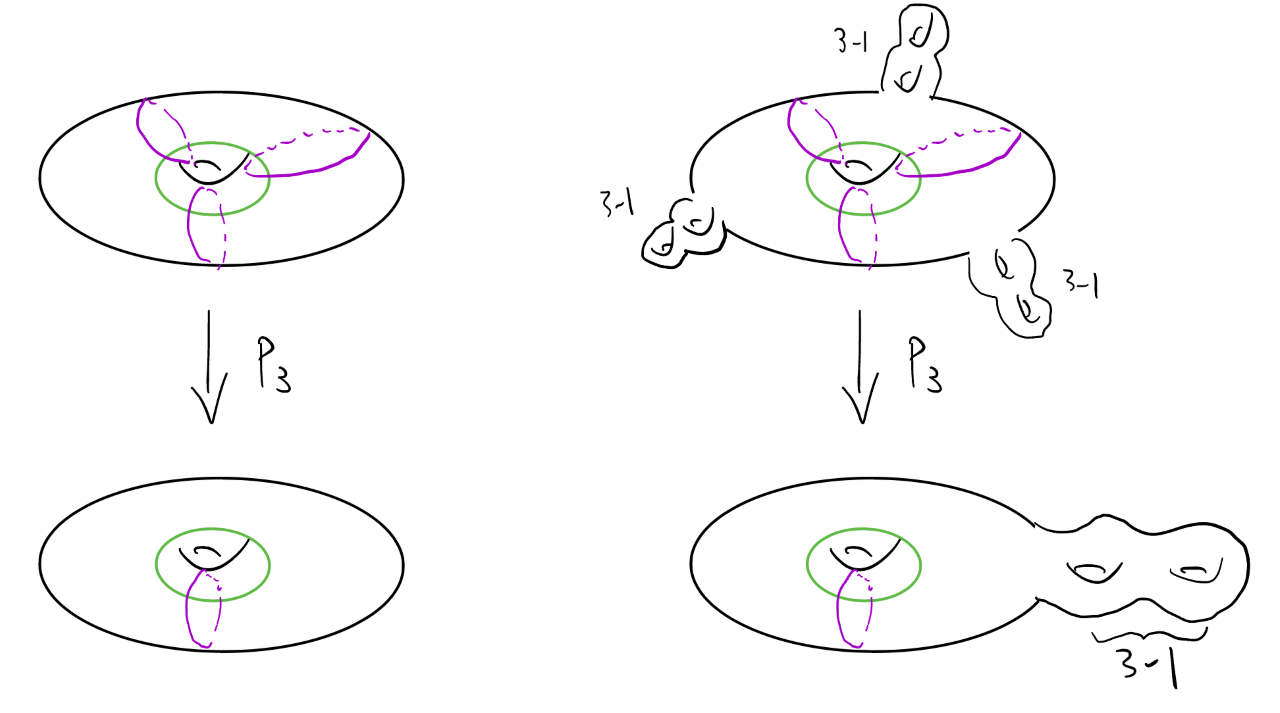
\includegraphics[width=0.8\textwidth]{./figures/covering_surf.png}
	\caption{Here we let $ g=n=3$.}
\end{figure}

\begin{problem}[7]
$ \rr P^{n}$ is $ S^{n}$ with antipodal points identified. But if we think of $ S^{n}$ as two disks glued along the equator, by the identification of antipodal point, we can forget about one disk and just keep track of how the remaining disk behaves. Then $ \rr P^{n}$ is also just $ D^{n}$ with boundary $ S^{n-1}$ antipodal points identified. That is, we glue $ D^{n}$ along $ \rr P^{n-1}$, so the attaching map $ f_{\partial D^{n}}$ is exactly the quotient map $ q_{n-1}: S^{n-1} \to \rr P^{n-1}$. We can do this inductively to obtain a CW-structure: starting with a single 0-cell, get a circle or $ \rr P^{1}$ using a single 1-cell, and glue a single 2-cell via quotient map as attaching map to the 1-skeleton $ \rr P^{1}$, then glue a single 3-cell via quotient map to 2-skeleton $ \rr P^{2}$, and so on. This way, we have the following chain complex:
\begin{align*}
	0 \xrightarrow{ \partial_{n+1}} C_n= \langle e^{n} \rangle \xrightarrow{ \partial _n}  C_{n-1} = \langle e^{n-1} \rangle \to \cdots \to C_2 = \langle e^{2} \rangle \xrightarrow{ \partial _2} C_1 = \langle e^{1} \rangle \xrightarrow{ \partial _1}  C_0 = \langle * \rangle \to 0    .
\end{align*}
For any $ k < n$, the attaching map  $ f_{\partial e^{k+1}} = q_k$. We obtain a map $ g_k : S^{k} \to S^{k}$ by composing
\begin{align*}
	\partial e^{k+1} \xrightarrow{ q_k} \rr P^{k} \to \rr P^{k} / \rr P^{k-1} \cong S^{k}.  
\end{align*}
Then to compute the degree of $ g_k$, we shall use local degrees. Take $ y \in \inte S^{k}$, Then $ g_k^{-1}(y)$ is pretty much just the antipodal $ x, a_k(x)$ (where $ a_k:S^{k} \to S^{k}$ is the antipodal map) that got quotient to  $ y$. Let $ U \ni x,V \ni a_k(x)$ be two disjoint neighborhoods that get identified to the same neighborhood of  $ y$, \emph{i.e.} $ U = a_k(V)$. Then since $ g_k|_V \circ a_k = g_k|_U$, we see that $ \deg (g_k|_U) = \deg((g_k|_V) \circ a_k) = \deg g_k|_V \deg a_k =(-1)^{k+1} \deg g_k|_V $.
\begin{align*}
	\deg g_k = \deg g_k|_U + \deg g_k|_V = (1+(-1)^{k+1}) (\deg g_k|_U) .
\end{align*}
Since $ \deg g_k|_U$ is $ \pm 1$,  $ \deg g_k = 0$ if $ k$ is even and  $ \pm 2$ if  $ k$ is odd. So  $ \partial_{k+1}(e^{k+1}) = \deg g_k e^{k}$. Rather we shift the index so $ \partial_k(e^{k}) = \deg g_{k-1} e^{k-1}$ is 0 for $ k$ odd and  multiplication by $ \pm 2$ for $ k$ even. The sign doesn't affect homology, so WLOG assume positive 2. Then for $ k<n$, we have $ \ker \partial_k = 0$ for $ k$ even and  $ \zz$ for $ k$ odd,  $ \im \partial_{k+1} = 0$ for $ k$ even and  $ 2\zz$ for  $ k$ odd. Thus for $ k<n$,
\begin{align*}
	H_k(\rr P^{n}) &= \ker \partial_k / \im \partial_{k+1}\\
		       &=\begin{cases}
			       0 & k \neq 0 \text{ even}\\
			       \zz /2 & $ k$  \text{ odd} \\
			       \zz & $ k = 0$
	\end{cases}
\end{align*}
If $ n$ is even, then  $ H_n(\rr P^{n}) = 0 / 0 =0$. If $ n$ is odd, then  $ H_n(\rr P^{n}) = \zz / 0 = \zz$.

For $ \zz /2$ coefficients, the changes are that $ \ker \partial_k = \zz /2$ for $ k$ odd, and  $ \im \partial_{k+1} = 0$ for $ k$ odd. Thus for $ k<n$,
\begin{align*}
	H_k(\rr P^{n}) &= \ker \partial_k / \im \partial_{k+1}\\
		       &=\begin{cases}
			       0 & k \neq 0 \text{ even}\\
			       \zz /2 & $ k=0$  \text{ or odd} \\
	\end{cases}
\end{align*}
If $ n$ is even, then  $ H_n(\rr P^{n}) = 0 / 0 =0$. If $ n$ is odd, then  $ H_n(\rr P^{n}) = \zz /2 / 0 = \zz /2$.


\end{problem}

\begin{problem}[8]
We start with a single 0-cell which generates $ \zz$. Suppose by induction we have built the $ (i-1)$-skeleton that gives the desired homology. For $ G_i$, since it is finitely generated abelian group, it is the direct sum of cyclic groups, either free as $ \zz$ or torsion as $ \zz /k$ for some $ k$. For each copy of $ \zz$, we attach $ e^{i}$ by the constant map to the 0-cell, \emph{i.e.} it gives an $ S^{i}$. For each $ \zz /k$ for some $ k$, do the same but also attached an $ e^{i+1}$ to the $ S^{i}$ by wrapping around $ k$-times. This way, we see that  $ C_i(X)$ is generated by one $ e^{i}$ per component of $ G_i$, plus one additional $ e^{i}$ per torsion component of $ G_{i-1}$. This is a wedge of $ S^{i}$ spheres (possibly filled). Clearly $ \ker \partial_i$ is the $ e^{i}$ that only come from $ G_i$, since the ones from $ G_{i-1}$ are all multiplication by $ k$ map which is injective. Similarly,  $ \im \partial_{i+1}$ is the image of multiplication by $ k$ maps into  $ e^{i}$ from torsion components, whereas the $ e^{i}$ from free part is not the boundary of any higher-dimensional cell so it remains free. That is, $ H_i(X) = G_i$.
\end{problem}

\begin{problem}[9]
It goes without saying that CW superscript is omitted. The cellular chain complex of $ X$ is
\begin{align*}
	0 \xrightarrow{ \partial_3}  C_2 = \langle \sigma, \tau  \rangle  \xrightarrow{ \partial _2}  C_1 = \langle \gamma  \rangle \xrightarrow{ \partial _1}  C_0 = \langle * \rangle \to 0  .
\end{align*}
Clearly $ X$ is path-connected so $ H_0(X) = \zz$, and $ \partial _1 = 0$ so $ \ker \partial _1 = \langle \gamma \rangle$. We see that
\begin{align*}
	\partial _2( \sigma) = 2 \gamma, \partial _2( \tau) = 3 \gamma
\end{align*}
Thus $ \partial _2( \tau - \sigma) = \gamma$ meaning $ \partial _2$ is surjective. Thus $ H_1(X) = 0$. Finally, by the split short exact sequence, $ \ker \partial _2 \cong \zz$. Since $ \im \partial _3 = 0$, we have $ H_2(X) = \zz$.
\end{problem}
\begin{problem}[10]
~\begin{figure}[H]
	\centering
	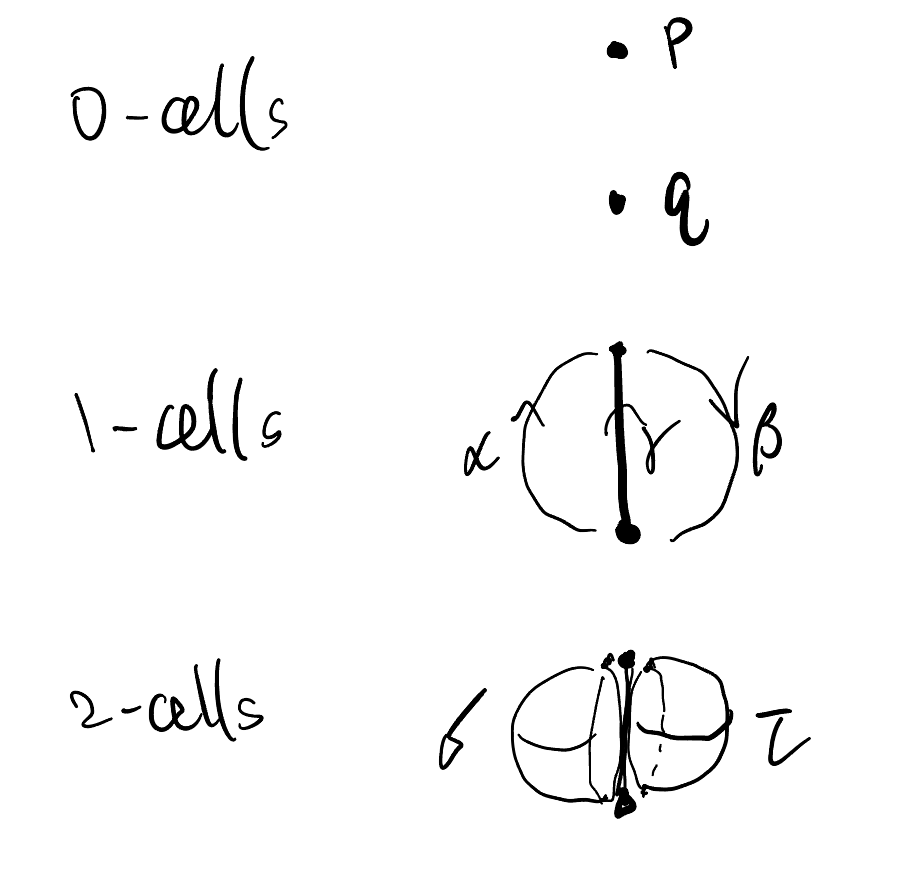
\includegraphics[width=0.5\textwidth]{./figures/5_10.png}
	\caption{Cell structure of $ X$.}
\end{figure}
The cellular chain complex of $ X$ is
 \begin{align*}
	0 \xrightarrow{ \partial _3} \langle \sigma, \tau \rangle \xrightarrow{ \partial _2} \langle \alpha, \beta, \gamma \rangle  \xrightarrow{ \partial _1} \langle p,q \rangle \to 0
\end{align*}
Again $ X$ is path-connected so  $ H_0(X) = \zz$. By taking the boundary with the orientations shown in the figure, we have $ \partial _1( \alpha) = - \partial _1( \beta) = \partial _1( \gamma) = p-q$. It follows that $ \ker \partial _1 = \langle \alpha+ \beta, \beta+ \gamma \rangle$. As shown in the figure, we see that $ \partial _2( \sigma) = \alpha+ \beta$ and $ \partial _2( \tau) = - \alpha- \beta$, so $ \im \partial _2 = \langle \alpha + \beta \rangle$ and $ \ker \partial _2 \cong\zz$. It follows that $ H_1(X) = \langle \beta+ \gamma \rangle \cong \zz$ and $ H_2(X) = \zz$.
\end{problem}
\end{document}
